\documentclass[12pt]{article}
\usepackage{graphicx}
\usepackage{parskip}
\usepackage{url}
\usepackage{float}
\usepackage{setspace}
\graphicspath{ {./pictures/} }
\onehalfspacing
\usepackage{subfig}

\begin{document}

\section{Risk Assesment}

To ensure the safety under operation and development of the drone, a risk assessment is created for the drone project, based on the Fine \& Kinney method \cite{finekinney}.

\begin{figure}[H]
    \begin{center}
    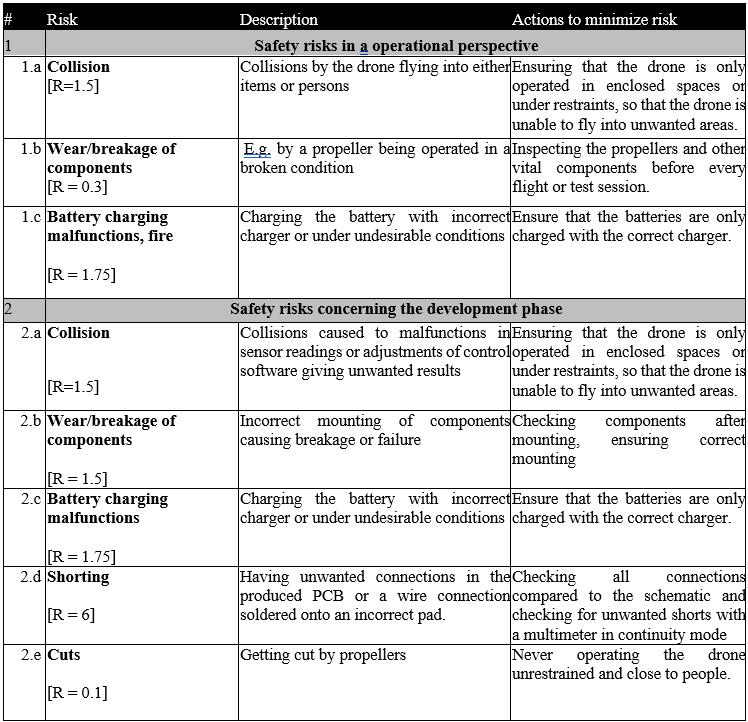
\includegraphics[scale=0.7]{Risk assesment table.png}
    \end{center}
    \caption{Motor control with MOSFET.}
    \label{fig:Mosfet_Control}
\end{figure}

Marked in all the risks are the risk scores calculated by the Fine \& Kinney method of Risk, Risk score = Probability * Exposure * Consequence. These risk scores are then compared in the risk clusters of the method, with five defined classes. After calculating the proposed risk ratings of the found risks, it’s apparent that all risks fall under the lowest factor of the Fine \& Kinney method of scores the: ‘Risk; Perhabs acceptable category’. 


\end{document}